\documentclass{bioinfo}

\copyrightyear{2016} \pubyear{2016}
\access{Advance Access Publication Date: XXX XXX XXXX}
\appnotes{XXXXXXXXXXXX}

%provided
\usepackage{url}
\usepackage{algorithm2e}
\usepackage{color}

% external package
\usepackage{amsmath}

% Numbering in eqns
\numberwithin{equation}{section}


% App defns
\def\haplo{{HaploForge}}
\def\hpainter{{HaploPainter}}

\definecolor{red}{RGB}{255,0,0}
\newcommand{\changes}[1]{\textcolor{red}{#1}}



\begin{document}

\firstpage{1}

\subtitle{Subject Section XXXX}

\title[\haplo{}]{\haplo{}: A Comprehensive Pedigree Drawing and Haplotype Visualisation Web Application}
\author[Tekman \textit{et~al}.]{Mehmet Tekman\,$^{\text{\sfb 1}}$, Alan Medlar\,$^{\text{\sfb 2}}$, Monika Mozere\,$^{\text{\sfb 1}}$, Robert Kleta\,$^{\text{\sfb 1}*}$, and Horia Stanescu\,$^{\text{\sfb 1}}$}
\address{$^{\text{\sf 1}}$Division of Medicine, University College London,  London,  NW3 2PF, UK and \\
$^{\text{\sf 2}}$Institute of Biotechnology, University of Helsinki, Helsinki, 00014, Finland.}

\corresp{$^\ast$To whom correspondence should be addressed.}

\history{Received on XXXXX; revised on XXXXX; accepted on XXXXX}

\editor{Associate Editor: XXXXXXX}

\abstract{\textbf{Motivation:} 
Haplotype reconstruction is an important tool for understanding the aetiology of human disease. Haplotyping infers the most likely phase of observed genotypes conditional on constraints imposed by the genotypes of other pedigree members. The results of haplotype reconstruction, when visualised appropriately, show which alleles are identical by descent despite the presence of untyped individuals. When used in concert with linkage analysis, haplotyping can help delineate a locus of interest and provide a succinct explanation for the transmission of the trait locus. Unfortunately, the design choices made by existing haplotype visualisation programs do not scale to large numbers of markers. Indeed, following haplotypes from generation to generation requires excessive scrolling back and forth. In addition, the most widely-used program for haplotype visualisation produces inconsistent recombination artefacts for the X chromosome.\\
%
\textbf{Results:} To resolve these issues, we developed \haplo{}, a novel web application for haplotype visualisation and pedigree drawing. \haplo{} takes advantage of HTML5 to be fast, portable and avoid the need for local installation. It can accurately visualise autosomal and X-linked haplotypes from both outbred and consanguineous pedigrees. Haplotypes are coloured based on identity by descent using a novel A* search algorithm and we provide a flexible viewing mode to aid visual inspection. \haplo{} can currently process haplotype reconstruction output from Allegro, GeneHunter, Merlin and Simwalk.\\
%
\textbf{Availability:} \haplo{} is licensed under GPLv3 and is hosted and maintained via Bitbucket.\\\
\textit{Web Application and Source Code:}\ \ \url|https://www.bitbucket.io/mtekman/haploforge|\\\
\textbf{Supplementary information:} Supplementary data is available from \textit{Bioinformatics} online.\\
\textbf{Contact:} \href{r.kleta@ucl.ac.uk}{r.kleta@ucl.ac.uk}\  % 
}

\maketitle

\section{Introduction}

\enlargethispage{15pt}
Linkage analysis, together with haplotype reconstruction, is used to identify putative locations of disease traits. Linkage analysis tests whether a given gene region co-segregates with the trait locus, whereas haplotype reconstruction infers the phase information that is lost during genotyping, i.e. the parental origin of each allele. In doing so, regions of interest can be found using linkage analysis and those regions delineated with inferred recombinations from haplotype reconstruction. Once a region has been identified, candidate genes can be selected for sequencing based on information from sequence databases (tissue-specific expression, homology, etc) or, if no candidate presents itself, all genes from the identified region can be screened for mutations using, for example, exome sequencing \citep{bockenhauer2012genetic}.

Many parametric linkage analysis programs also perform haplotype reconstruction based on maximum likelihood. However, to integrate these analyses together requires advanced visualisation methods to intuitively display haplotypes together with the pedigree structure and to colour haplotypes based on identity by descent (IBD).


There are many programs available for haplotype visualization, \changes{such as the highly cited \hpainter{} \citep{hpaint} as well as the more recent Family Genome Browser \citep{familygenomebrowser}, the former being the target of our critique due to the better compatible feature-overlap against our own application}. However, our experience with \hpainter{} has shown that viewing haplotypes inline with the pedigree does not scale to large numbers of markers. Indeed, to compare haplotypes between generations requires excessive scrolling and the user has to re-identify the same region of interest over and over again in each successive generation. In addition, \hpainter{} does not always correctly display which alleles are IBD, creating inconsistent recombination artefacts for the X chromosome. As shown in Figure~\ref{fig:hpainterx}, the last generation of individuals (particularly 206130, 206121 and 206117) appear to have undergone multiple recombinations within a relatively short genetic distance (< 1 cM).

\hpainter{} fails to properly account for the fact males have only a single X chromosome and, therefore, can appear to inherit from their father or even from an undisplayed paternal allele (see blue allele in individuals 206121 and 206117 in Figure~\ref{fig:hpainterx}).

To resolve these issues we present \haplo{}, a novel web application for haplotype visualization and pedigree drawing. \haplo{} is designed specifically for navigating high numbers of markers, providing a more intuitive viewing mode compared to other programs. 
Secondly, we present a novel A* search-based method that ensures IBD information is correctly displayed for all chromosomes, including the X chromosome.

Finally, \haplo{} is web-based and therefore runs in any HTML5-compatible web browser and does not require local installation. Despite being web-based, it is fast and the user experience is similar to a native application, utilizing menus and a drag and drop interface.

\begin{figure}[!tpb]
	\centerline{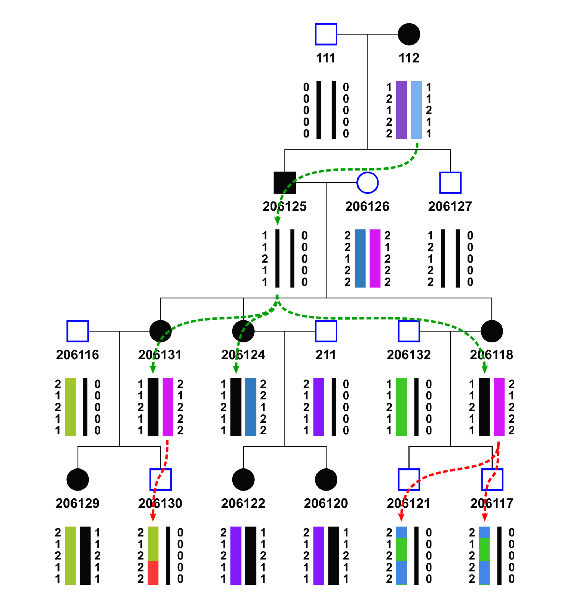
\includegraphics[scale=1]{hpainter_inheritance_small.4.eps}}\caption{\hpainter{} visualisation of a five marker X-linked analysis. Colours indicate identity by descent. Arrows are overlayed to show the true flow of genetic data based on genotypes, with green showing inconsistent colouring between successive meioses and red showing erroneous inheritance.}\label{fig:hpainterx}
\end{figure}



\section{Approach}

% overview of features of program
\haplo{} is a comprehensive web application for haplotype visualisation and pedigree drawing.\

Here we will enumerate and expand upon the core features.

\subsection{Pedigree Drawing}

\begin{figure}[!tpb]
	\centerline{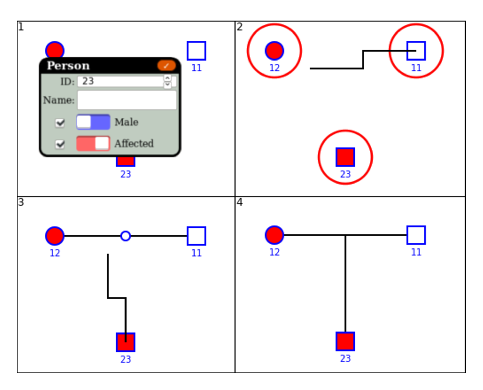
\includegraphics[scale=1]{pedcreate.4.eps}}\caption{Pedigree drawing view show the four stages of creating a pedigree: (1) Adding individuals and modifying their properties, (2) Joining mates with a mateline to anchor points made visible with red circles, (3) Joining offspring to their parents through a childline to anchor points made visible with white circles, (4) Completing a trio.}\label{fig:pedcreate}
\end{figure}
	
Pedigrees are drawn with a simple drag and drop interface, and are compliant with the Pedigree Standardization Work Group (PSWG) specification \citep{pswg1,pswg2}. The standard is already familiar to clinicians and allows individuals in the pedigree to be annotated with patient metadata. 

Individuals are added to the pedigree either through context-dependent sidebars or user-customizable keyboard shortcuts, and the properties of that individual (sex, affection status, etc) can then be edited from a dialog box. Relationships between individuals are added by drawing {\it matelines} and {\it childlines}. Matelines indicate marriages and childlines connect children to their parents' mateline. Lines snap to context-dependent anchor points that become visible when adding relationships (Figure~\ref{fig:pedcreate}). Both members of each mateline are vertically aligned with one another and move together as a single unit. Siblings bound to the same mateline are similarly aligned automatically.

Projects can contain multiple families, and complex consanguineous relationships are automatically detected and represented with double-lines. Pedigrees can be loaded from and saved to local browser storage. Pedigrees can be imported and exported in standard LINKAGE (pre-makeped) format.
	
\subsection{Haplotype Visualisation}

\begin{figure}[!tpb]
	\centerline{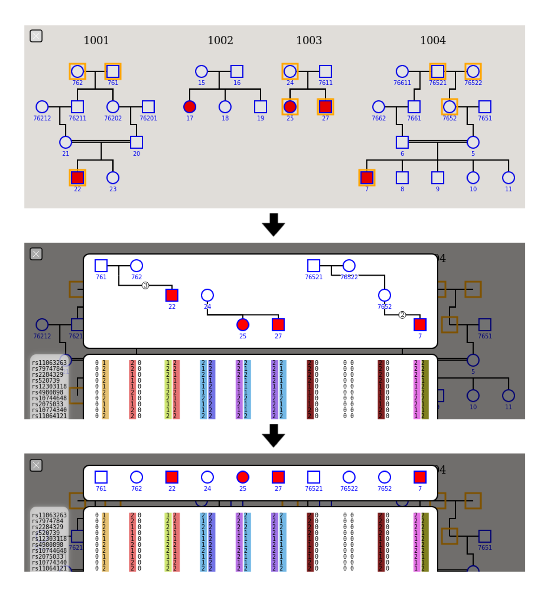
\includegraphics[scale=1]{dos2.4.eps}}\caption{(Top) Selection view enabling the subselection of individuals across multiple pedigrees. (Middle) Comparison view displaying the haplotypes of selected individuals, connected by lines indicating their degrees of separation from one another. (Bottom) Comparison view representing the same genotypes but with individuals vertically aligned.}\label{fig:dos}
\end{figure}

\begin{figure}[!tpb]
	\centerline{\includegraphics[scale=1]{all_in_one.4.eps}}\caption{Modes of interaction: (Top) scrolling the genotypes in the comparison view by dragging and dropping the haplotypes, updating the marker positions in the chromosome overview; (Middle) adjusting the viewport by manually specifying a locus of interest between two markers; (Bottom) resizing the viewport by dragging the upper or lower handle on the chromosome overview, along with a Shift keyboard modifier for permitting slower movement for precision. A viewport larger than the size of the window can be scrolled using the mouse wheel, but the default behaviour can be reverted by holding Ctrl and dragging one of the handles to snap the viewport back to the window size.}\label{fig:viewportmanip}
\end{figure}	

		
While \hpainter{} visualises haplotypes inline with the pedigree, in \haplo{} haplotypes are displayed in a separate viewing mode.

Selected individuals are aligned horizontally and grouped by family. Haplotypes are displayed underneath each individual, allowing for side-by-side comparison, irrespective of generation. The relatedness of individuals can be optionally displayed, with relationship lines stating their degree of separation (see Figure~\ref{fig:dos}). 

Haplotypes are displayed within a viewport that defines the locus of interest across the genotypes of all selected individuals, the contents of which are outlined on the chromosome overview. The overview consists of a red vertical bar representing the entire length of the chromosome, and it is overlayed with a region indicator which has a height and position that maps to the size and location of the viewport on the chromosome.

\pagebreak
The viewport can be manipulated by a variety of different interactions as shown in Figure~\ref{fig:viewportmanip}: dragging the region indicator in the overview, scrolling the mouse wheel over the genotypes, or using keyboard shortcuts for fast (PageUp/PageDn) and slow (Up/Down arrows) movement. Precise modes of adjustment are also provided; dragging and releasing haplotypes at a desired vertical position, shifting to the next/previous point of recombination, or specifying a pair of markers from a dropdown list.

The chromosome overview also allows for the size of the viewport to be adjusted through dragging the top and bottom handles on the region indicator as shown in Figure~\ref{fig:viewportmanip} (Bottom). By default, the size of the viewport is locked to the size of the window. However, if the viewport is made bigger than the window, it can be scrolled using the mouse wheel.

\subsection{IBD Colouring}

In \haplo{}, haplotypes are coloured by IBD by converting the task of resolving ambiguous parentage into a path-finding problem and performing A* search to determine the path with least recombinations. A* search is an efficient path-finding algorithm used in real-time mapping applications \citep{algfoor2015comprehensive}.

In a connected graph with weighted edges, an optimal path between two nodes is found by minimising the total edge cost. 

A* search is a best-first search algorithm that, in the process of finding the optimal path, maintains a ``frontier'' of nodes from which the node deemed most likely to be the next intermediate node on the path to the target node is selected. The search procedure is admissible on condition that the estimated cost to the target node is not greater than the true cost from the next intermediate node to the target node, under the following heuristic: $f(n) = g(n) + h(n)$, where $n$ is an intermediate node on the path, $g(n)$ is the cumulative cost of the path (from start node to $n$), and $h(n)$ is the heuristic that estimates the lowest cost from $n$ to the target node \citep{astar}.

In a genomic context this can be conceptualised as a multi-layer network graph, where edges only exist between consecutive layers. Each layer represents an individual marker locus, and each node a distinct founder allele (Figure~\ref{fig:pathfind}). The algorithm traverses from one end of a chromosome to the other under the heuristic of minimizing the number of recombinations. A maximum of $2f$ nodes are possible in each layer, where $f$ is the number of founders. This number is often far smaller due to the manner in which the graph is initialised (see Section~\ref{alg:initial}).

\subsection{File Format Support}\label{fileformat}

\haplo{} accepts phased genotypes from both binary markers (SNPs) and polymorphic markers (e.g. VNTRs and STRs), in vertical or horizontal pre-MAKEPED or modern LINKAGE-based formats with chromosome pairs delineated on adjacent lines. 

\haplo{} can additionally utilise supplementary gene flow information output by specific programs. Some applications incorporate this information within the main haplotypes output file, whereas others provide it in a supplementary file. Merlin \citep{merlin}, for example, outputs founder alleles in a file called \path{gene.flow}. Allegro \citep{allegro} and SimWalk \citep{simwalk} both output the optimal descent graph, stating the gene flow between generations. The haplotypes from GeneHunter \citep{kruglyak1996} and Merlin do not include sex data, requiring it be inferred through parentage for all but the last generation whose sex is declared unknown. This information can be provided separately. Further marker data (e.g. SNP ID, genetic distance, etc) is displayed upon discovery and preserved across successive sessions in local storage.


\begin{methods}

\section{Methods}

\begin{figure}[!tpb]
	\centerline{\includegraphics[scale=1]{path_finder.4.eps}}\caption{(Top) A multi-layer network graph depicting five founder alleles as uniquely coloured nodes within a marker locus stretching from $m_i$ to $m_{i+5}$. Black arrows depict desired contiguous founder-allele stretches, and grey arrows indicate recombinations from one founder-allele to another. (Bottom) Six possible routes explored by the search algorithm, with contiguous stretches being rewarded $+1$ to the total path sum. The first route has the largest path sum of 4 and is the most optimal path in the range considered.}\label{fig:pathfind}
\end{figure}


%\vspace{-1cm}
\subsection{Web Technology}

\haplo{} is implemented using HTML5 and JavaScript. Unlike other haplotype visualisation programs that require local installation (including installation of dependencies), \haplo{} runs in any compliant web browser. Features like A* search IBD colouring (described in detail in Section~\ref{astarsearch}) make use of JavaScript's typed arrays to eliminate the redundancy of the default numeric float type, compacting large numeric sets into small 8 bit decimal arrays. Fast 2D graphics rendering is performed using the HTML5 canvas-based {KineticJS library (\url{http://kineticjs.com})}. KineticJS renders graphics to layers which are implemented as separate canvas elements. 

\enlargethispage{0.5cm}

\haplo{} uses two layers for drawing operations, each acting either as a framebuffer or backbuffer where necessary to limit the number of redraw operations.

Animation is used to transition between the pedigree drawing and haplotype comparison modes. Visual effects can be disabled if, for example, the browser does not support hardware acceleration and performance is degraded. At time of writing, Webkit-based browsers (Chrome, Safari) offer better performance than the Gecko-based Firefox.

\subsection{A* search IBD Colouring}
\label{astarsearch}

\begin{figure}[!tpb]
	\centerline{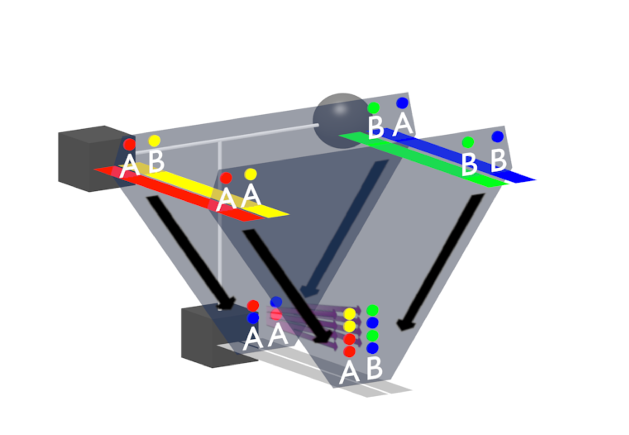
\includegraphics[scale=1]{graph_and_path2.4.eps}}\caption{Parent-Offspring trio for a 2-marker locus. The two vertical layers display the independent founder-allele group initialisation occurring at each marker locus, with the proliferation of founder-alleles (coloured dots) from parent-to-offspring under valid genotype configurations. The A* search process then bisects these layers for each non-founder allele, to maximize the length of a contiguous founder-allele.}\label{fig:graphpath}
\end{figure}

The procedure to ensure that haplotypes are coloured appropriately to reflect identity by descent occurs at the level of parent-offspring trios, ordered through a top-down pass of the pedigree ensuring that offspring are not processed before their parents.
For each trio, processing is split into two distinct phases: initialising the graph, and determining the optimal path using A* search.


\subsubsection{Graph Initialisation}
\label{alg:initial}

Founder alleles are inherited by non-founders transitively via their parents. For each non-founder allele, we define the set of all valid founder allele assignments that could be made based on the genotypes of the parents. This is termed the {\it founder allele group}. In the trivial case, the founder allele graph only contains a single element and, therefore, the founder allele inherited is unambiguous. However, given that there tend to be multiple valid paths by which a given allele could have been inherited, there will often be multiple possible founder alleles.

Although our implementation of A* search requires phased genotypes, (i.e.~resulting from haplotype reconstruction, see next section), 
the graph initialization procedure does not make use of the phase information, relying solely on the founder allele groups as shown in Figure~\ref{fig:graphpath}. 

\subsubsection{Finding the Optimal Path}

\enlargethispage{0.5cm}

During graph initialisation, genotypes are processed vertically, parent-to-offspring, to populate the founder allele groups at each marker locus. 
The A* search algorithm traverses the chromosome, from marker to marker, to find the optimal path defined by the lowest cost combination of founder allele assignments.
The search operates under the heuristic of maximising contiguous stretches (or \textit{paths}) of the same founder allele across multiple marker loci, minimizing the number of recombinations. The branching nature of the search requires we consider multiple paths, each of which expands the frontier of possible founder allele groups. Valid paths are restricted to those that meet minimum stretch requirements and fall within accepted founder allele assignments outlined in Algorithm~\ref{alg:astar}.

The founder alleles assigned during graph initialisation do not state whether they are inherited maternally or paternally. To address this, we define a \textit{parental exclusion set} that encapsulates all the founder alleles present in either maternal or paternal alleles. The algorithm then selects from these sets to determine where the allele originated from. In the case of a consanguineous relationship, each maternal and paternal exclusion set subtracts against the union of both sets to permit the inclusion of shared groups.

A maximum working set of eight examined paths are expanded upon with paths added/removed according to the number of recombinations. Paths with the same number of recombinations are included but discounted from the working set in order to encourage path diversity.
Once an active path reaches the final locus, it is moved into the set of complete paths from which the path with the lowest number of recombinations will be selected at the end of the procedure.


%%% Pseudocode
\begin{algorithm}[!t]
\label{alg:astar}
\SetLine\

\Begin{

\textit{X} $\leftarrow$ parental exclusion set of illegal founder-alleles

\textit{frontier} $\leftarrow$ set of active paths, initialized to first founder-allele

\textit{complete} $\leftarrow$ set of completed paths, initialized as empty

\While{frontier > 0}{

   \textit{p} $\leftarrow$ first path in \textit{frontier}
   
   \textit{F} $\leftarrow$ set of founder-alleles at marker locus \textit{\textnormal{size}(p)+1} 
     
   \For{f $\in$ F}{
           
      \textit{s} $\leftarrow$ perform lookahead and count contiguous stretch of \textit{f}
      
      \If{(s > \textit{minStretch}) \textnormal{and} (f $\notin$ X)}{
          \textit{e} $\leftarrow$ extend path \textit{p} by length \textit{s} with founder-allele \textit{f}
      
	      \eIf{\textnormal{size}(e) > \textnormal{size}(markers)}{
    	  	push \textit{e} to \textit{complete}
	      }{
    	  	push \textit{e} to \textit{frontier}
	      }      
      }
   }
   sort \textit{frontier} by desc. length and truncate up to \textit{maxNumPaths}
}
sort \textit{complete} by desc. number of recombinations

\Return{\textnormal{first path in} \textit{complete}}


}
\caption{A* search upon a single chromosome pre-initialised with a set of potential founder-alleles at each marker locus.}
\end{algorithm}
%%%%%%

\begin{figure}[!tpb]
	\centerline{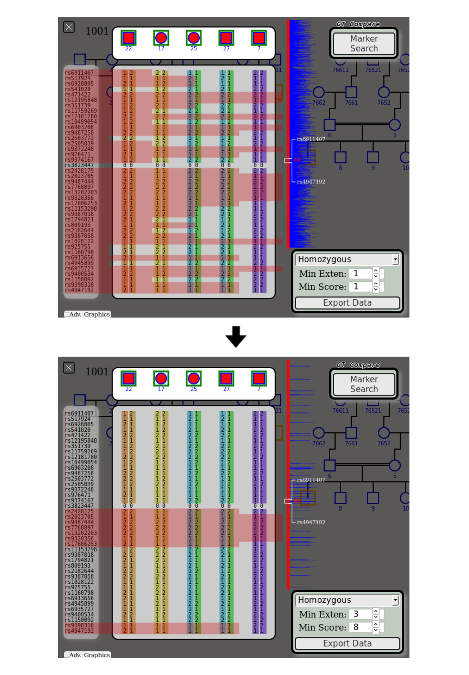
\includegraphics[scale=1]{homology.4.eps}}\caption{Comparative view displaying identity scores under a homozygous context, with (Top) no filtering and (Bottom) a minimum score threshold of 8 and a minimum peak size of 3 markers. Scores are overlayed on both the genotypes and the chromosome overview.}\label{fig:homology}
\end{figure}



\subsection{Comparative Analysis}

The purpose of haplotype visualisation is to help distinguish between loci whose segregation is concordant with the disease trait from those that are not. In such regions there will be a clear distinction in IBD information between affected and unaffected individuals. To give researchers an overview of their data, \haplo{} defines a per locus score based on the extent to which haplotypes for affected individuals differ from unaffected individuals

The scoring function is specified by the type of zygosity selected by the user. Under a heterozygous setting, only a single allele from each individual would need to match. For homozygousity and compound heterozygousity, individuals need to have the same set of alleles, with the former requiring those alleles additionally be homozygotes.

\pagebreak
This is defined explicitly in the equations below, where for a given marker locus \textit{m} and family \textit{f}, scores are generated for each of the three zygosity scenarios as follows:\
\begin{gather}
\text{SCORE (\textit{m, f})} = \sum_{i}{g(A_i,m)} - \sum_{j}{g(U_j,m)}\\
\
\begin{flalign}
\nonumber\
\text{where:}&\\
\nonumber\
& A = \text{Affecteds in }f,\ \ \ U = \text{Unaffecteds in }f\\
\nonumber\
& A_0 = \text{Initially selected affected individual in }f\\
\nonumber\
& H_{p,m} = \text{Set of haplotypes for individual \textit{p} at locus \textit{m}}\\
\nonumber\
\text{and }g \text{ refers} & \text{ to one of:}\\
\nonumber
& \ het(p,m) = \begin{cases}
	1 ,& \text{if } \exists\ h\ \epsilon\ H_{p,m}\ : h\ \epsilon\  A_{0,m}\\
	0 ,& \text{otherwise}
		\end{cases}\\
\nonumber\
& chet(p,m) = \begin{cases}
	1 ,& \text{if } H_{p,m} = A_{0,m} \text{ and } |A_{0,m}| > 1\\
	0 ,& \text{otherwise}
		\end{cases}\\
\nonumber
& hom(p,m) = \begin{cases}
	1 ,& \text{if } H_{p,m} = A_{0,m}  \text{ and } |A_{0,m}| = 1\\
	0 ,& \text{otherwise}
		\end{cases}\\
\nonumber
\end{flalign}
\end{gather}

\vspace{-10pt}
The graphical representation is then the summation of this score across all families, to be overlayed upon both the genotypes and the chromosome overview (Figure~\ref{fig:homology}). Additional refinement can be performed by the user such as specifying a minimum score threshold to filter out less significant peaks, and setting a extension lower-bound to yield broader peaks.

\end{methods}


\pagebreak
\section{Discussion}

\haplo{} provides a unified environment to create, analyse, and visualize pedigrees together with their associated haplotypes. Pedigree creation allows for large families to be drawn using the mouse and exported or saved to local storage between sessions. Processing for IBD colouring is highly efficient and the results viewable across multiple families simultaneously. We provide several methods to inspect the displayed haplotype data including: displaying haplotypes between user-specified flanking markers, skipping between recombination points and scoring by haplotype consistency with the disease model.

\subsection{Path-finding approach}


The A* search processes each sister chromatid independently of one another, however the correct resolution of one chromatid depends upon the correct resolution of the other due to the mutual-exclusivity of the maternal or paternal exclusion set they are processed against. Due to the non parent-specific manner in which \haplo{} initialises founder-alleles, this may prompt the A* search to reprocess both chromatids with swapped parental exclusion sets if a path cannot be determined initially. 
Though seemingly costly, the lack of strict phasing during the founder-allele group initialisation stage and the serial processing of chromatids provides a greater flexibility in resolving a larger scope of genetic disorders. 
In the future this could be adapted to explore monosomy, trisomy, and tetrasomy cases.


\subsection{Visualisation Accuracy}

The haplotype visualisation performed by \haplo{} was compared with \hpainter{}. For all autosomal pedigrees analysed, the same points of recombination were identified from Allegro (ihaplo.out), GeneHunter (haplo.chr), Merlin (merlin.chr), and Simwalk (HEF.ALL) output files. Beyond the simple pedigrees, we have used \haplo{} with four non-trivial families: autosomal dominant (27 members, 23-bit); a highly consanguineous autosomal recessive (24 members, 29-bit); and an X-linked dominant (17 members, 15-bit).

Fig~\ref{fig:xcomp} provides a side-by-side comparison of the same X-linked pedigree shown previously (Figure~\ref{fig:hpainterx}), but showing a larger number of markers, where only \haplo{} shows the correct IBD colouring. \hpainter{} normally displays haplotypes inline with the pedigree, but this was modified in Figure~\ref{fig:xcomp} for comparison.


\begin{figure}[!tpb]
	\centerline{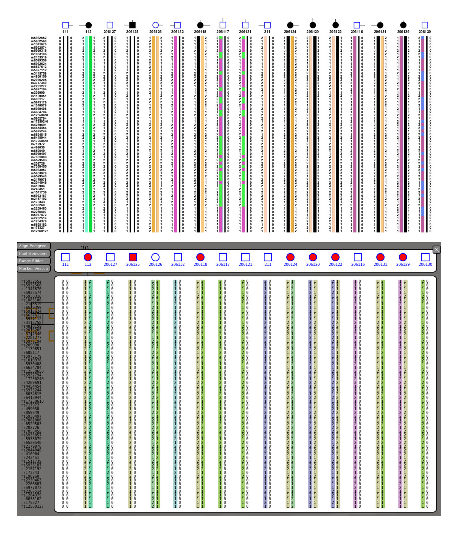
\includegraphics[scale=1]{x_compare.4.eps}}\caption{A comparison of the X-linked dominant pedigree showing a mid-region of chrX spanning 72 markers. (Top) \hpainter{} with output modified only for horizontally alignment, and (Bottom) \haplo{} showing all members via default comparison view.}\label{fig:xcomp}
\end{figure}


\subsection{Comparison with Other Haplotyping Software}

\changes{\hpainter{} dominated much of prior discussion due to the better feature-overlap with \haplo{} (pedigree creation, in-house haplotype recombination detection and rendering), but various different programs were considered for comparison.}

\subsubsection{Family Genome Browser}

\changes{The recent Family Genome Browser (FGB) \citep{familygenomebrowser} is a hybrid Java/Javascript web and desktop application which visualizes variant data under a pedigree context and hosts many useful features such as potential recombination events, IBD visualization, parent-of-origin highlighting, and linkage disequilibrium (LD) annotations. Java is not required to run the application within the browser, suggesting that the Java component operates on the server and the client interacts with the Javascript front-end, which in itself relies on heavy frameworks such as \textit{jQuery} and \textit{Raphael}. The desktop deployment of their utility is a Java servlet wrapper of their web-based version.}

\changes{In contrast, \haplo{} is written entirely in Javascript and relies only on the KineticJS framework for graphics rendering. Drawing functions are accessed independently through an interface in a manner that would permit for the framework to be easily exchanged in favour of another, without having to compromise the rest of the code. By having no actual dependents, \haplo{} can be effortlessly deployed to any platform (Web, Desktop, Mobile) that supports a web-engine under a myriad of different coding strategies (Java, C++, Python, Perl, etc).}

\changes{The FGB also seems to be primarily sequence-variant fixated in the formats that it accepts (VCF / CGF / BED), but does not appear to process any common haplotype formats (see Section~\ref{fileformat}), suggesting that recombination events are limited to examining the pre-set phasing of variants within variant data and evaluating haplotypes on a marker-by-marker basis as opposed to a more global scope. The parent-of-origin highlighting feature indicates the founder of a given marker-variant, but this is implicitly represented in \haplo{} via distinct colouring where the origin of a given non-founder allele block is inferred by the colouring of the founder allele it originated from (e.g. a small RED allele block in a last-generation individual can be traced back to the entire RED allele in a first-generation founder).}

\changes{The annotation of LD data makes sense in a variant-centric analysis but less so in a more haplotype/IBD driven context, and \haplo{} was originally developed to explore how alleles segregated within a pedigree setting only}.


\subsection{Privacy}

\haplo{} operates entirely \textit{in-situ} within the browser, with analyses restricted to a single user. In the interests of scientific collaboration, it is likely that the end-user would want to share their analysis with other researchers working on the same project. Due to the sensitivities of patient data, however, as well as the possibility of identifying individuals based on pedigree structure alone, \haplo{} was designed with the intention of not requiring any client-server communication after the web application has loaded. \changes{Server-side processing required by other web applications (such as FGB) are not a concern in \haplo{}, removing any need for the end-user to transfer sensitive patient data onto remote servers via potentially insecure protocols}. The discretion of patient data is ultimately left to the user, and we provide the option to strip patient names and other annotations on export.

\enlargethispage{1.8cm}

\subsection{Future Work}

\haplo{} was built on top of KineticJS because of its stability; active development being frozen since 2014. However, in order for \haplo{} to benefit from performance improvements it will need to migrate to one of the primary alternatives, either {ConcreteJS (\url{http://concretejs.com/})}, by the author of KineticJS or {KonvaJS (\url{https://github.com/konvajs/})} that both other distinct features and advantages that will need to be evaluated.

The inclusion of LD annotations would provide broader population insights to haplotype analysis from the default family-only setting. TODO


Future versions of \haplo{} will aim to integrate the visualization and creation modes to provide more flexibility, for example, to allow for modifying an existing pedigree after haplotype data is loaded.
Additional features could include SVG export and selective visualisation of multiple regions to help produce publication quality figures.

\enlargethispage{1.8cm}

\vspace{-0.5cm}
\section*{Acknowledgements}

R.K. is supported by St. Peter's Trust for Kidney, Bladder and Prostate Research, the David and Elaine Potter Charitable Foundation, Kids Kidney Research, Garfield Weston Foundation, Kidney Research UK, the Lowe Syndrome Trust, the Mitchell Charitable Trust, and the European Union, FP7 (grant agreement 2012-305608 "European Consortium for High-Throughput Research in Rare Kidney Diseases (EURenOmics)".\\\
\\
\noindent
\textit{Conflict of interest:} None declared.

\vspace{-0.2cm}
\bibliographystyle{natbib}
\bibliography{smallbib}

\end{document}
